\subsection{AstEpi parametric equation}

\begin{table}[ht]
	\begin{center}
		\begin{tabular}[top]{ |p{16.0 cm}| }
			\rowcolor{LIGHTCYAN}			
		%%	\hline \multicolumn{1}{|c|}{\textbf{Part 3/5 Circle and AstEpi parametric curves}} \\ [1.0ex]

					
            \rowcolor{LIGHTCYAN}
			\hline \textbf{No. 6 - AstEpi = Sum of (Astroid + Epicycloid) parametric curves}\\
			
			\begin{eqnarray}
				tiny & = & 1.0\tenpow{-10} \nonumber \\
				x(u) & = & 40[\sin(2\pi u)]^3 + 50\cos(2\pi u + tiny) - 10\cos(10\pi u -tiny) \nonumber \\
				y(u) & = & 40[\cos(2\pi u)]^3 + 50\sin(2\pi u + tiny) - 10\sin(10\pi u -tiny) \nonumber \\
				u & \in & [0.0, 1.0] \nonumber
			\end{eqnarray}
			
			
			Closed loop\\
			Overall Three loops, all convex curves \\
			Reflection x-axis: non-symmetrical\\
			Reflection y-axis: non-symmetrical\\
			\frame{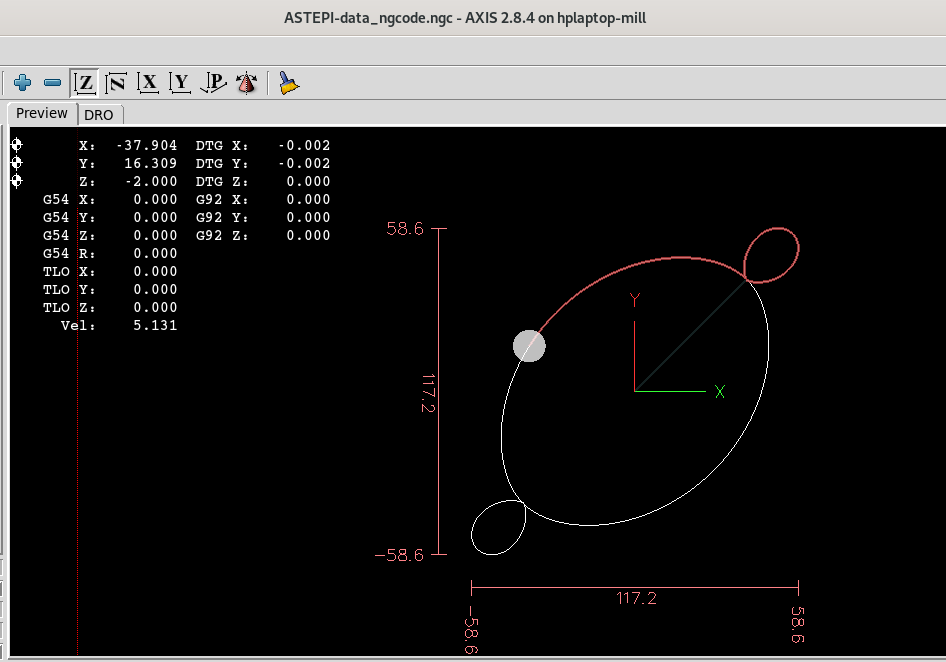
\includegraphics[width=0.560\textwidth]{./07-images/img-Ch5/ASTEPI-Axis.png}}
			\frame{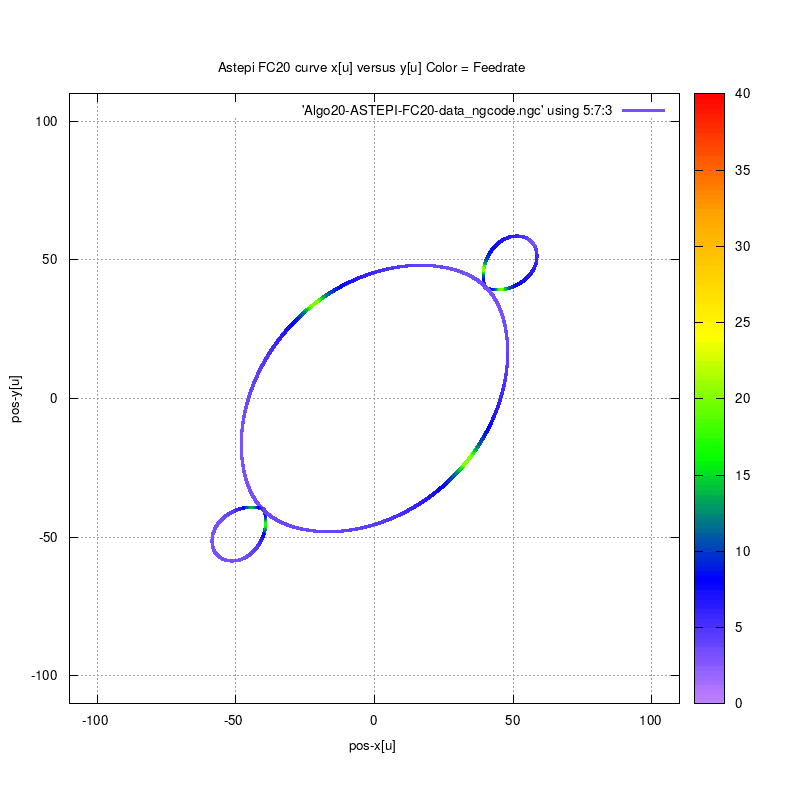
\includegraphics[width=0.395\textwidth]{./07-images/img-Ch5/ASTEPI-Feedrate.png}}\\
			
			\hline
		\end{tabular}
		\caption{Astepi equation and dimensions}		
		\label{table:Astepi equation and dimensions}
	\end{center}
\end{table}  
